\graphicspath{{chapters/laboratory/05/images}}
\chapter{Ancestry}

\section{Introduction}

	\subsection{Population stratification}
	The degree of admixture and population of origin identification is important for population stratification correction in:

	\begin{multicols}{4}
		\begin{itemize}
			\item GWAS studies.
			\item Ancestry.
			\item Migration pattern studies.
			\item Precision medicine.
		\end{itemize}
	\end{multicols}

	\subsection{Methods}

		\subsubsection{Principal Component analysis based methods}
		In principal component analysis methods the low-dimensional projection of the data allows to maximally retain variance-covariance structure among the genotypes.
		Fast algorithms are available to solve the problem, but interpretation might be non-trivial.
		Some examples are:

		\begin{multicols}{4}
			\begin{itemize}
				\item EIGENSTRAT.
				\item SMARTPCA.
				\item LASER.
				\item EthSEQ.
			\end{itemize}
		\end{multicols}

		\subsubsection{Model based methods}
		The explicit generative model for the data is based on Hardy-Weinberg equilibrium and linkage equilibrium.
		Probabilistic methods estimate ancestry information from inference of the best model parameters that fit the data.
		Some examples are:

		\begin{multicols}{4}
			\begin{itemize}
				\item STRUCTURE.
				\item FastSTRUCTURE.
				\item ADMIXTURE.
				\item FRAPPE.
			\end{itemize}
		\end{multicols}

\section{SMARTPCA}

	\subsection{Introduction}
	SMARTPCA is a PCA-based method specifically developed for SNPs data.
	The input is the genotype of $N$ SNPs for $M$ individual in a tool-specific format.
	It is also possible to apply a conversion from the PED format.
	The genotype data is always encoded in a matrix, the difference between data formats involves the SNP information.

	\subsection{PED format}
	A PED file contains a:

	\begin{multicols}{2}
		\begin{itemize}
			\item Genotype file: information about the individual in the first $6$ lines, like ID, sex, affection and genotype.
			\item Map file: chromosome, marker ID, genetic distance and physical position.
		\end{itemize}
	\end{multicols}

	\subsection{Output}
	SMARTPCA converts the two files of the PED format in a proprietary one.
	Then monomophic and suboptimal SNPs are excluded from the PCA.
	The output is a table of an user defined number of eigenvector.
	The result will be a plot with clusters of individuals divided according to geographical origin.
	A more detailed analysis could be performed increasing the number of individuals.

\section{fastSTRUCTURE}

	\subsection{Input}
	The input for fastSTRUCTURE is the genotype of $N$ SNPs for $M$ Individuals in BED, BIM or FAM formats.
	BED is a binary format with genotype data, while BIM and FAM contains SNPs and samples information.

	\subsection{Output}
	Data is clustered and for each individual the amount of genetic background coming from a specific population is determined.
	The method is supervised, with a number of cluster given as input beforehand.
	The output is a matrix containing a probability value for each of the inferred cluster for each individual.
	The final representation allow to visualize patterns of ancestry.

\section{EthSEQ}

	\subsection{Introduction}
	Starting from the idea of PCA methods, model-based reasoning is applied.
	The starting point is a set of genotype data and a reference model with a set of individuals from known populations, creating an aggregated model.
	After the PCA it is easier to quantify the level of admixture and population of origin exploiting the reference data.
	The EthSEQ pipeline is described in figure \ref{fig:ethseq}.

	\begin{figure}[H]
		\centering
		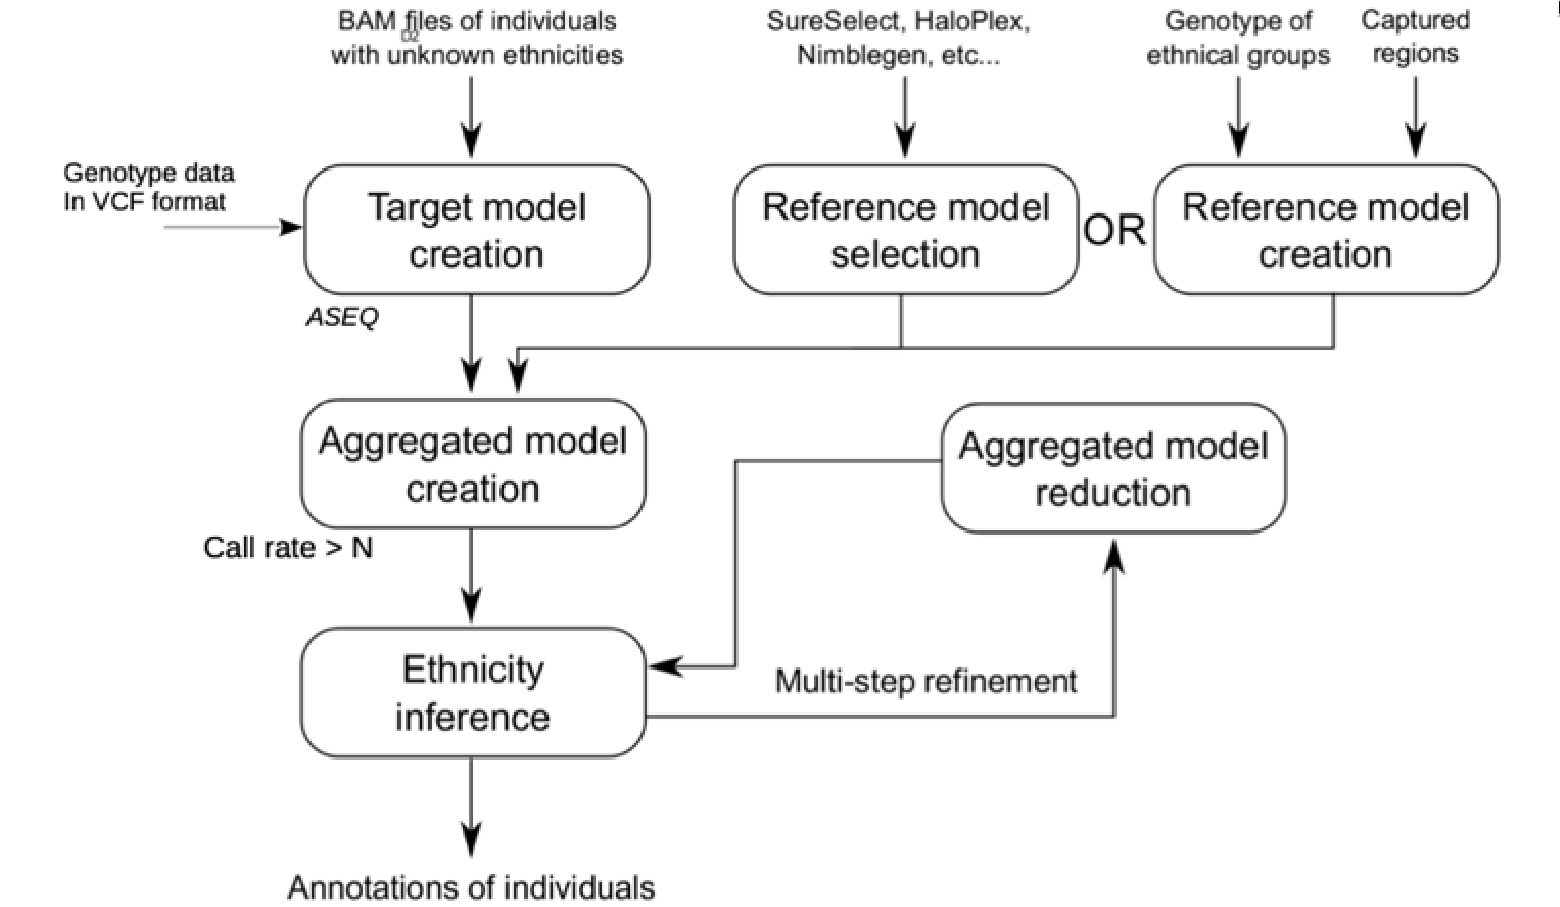
\includegraphics[width=\linewidth]{ethseq}
		\caption{EthSEQ pipeline.}
		\label{fig:ethseq}
	\end{figure}


	\subsection{Analysing sequencing data}
	EthSEQ is design to analyse whole exome or targeted sequencing data from BAM or vcf file.
	The PCA in 3D shows that exploiting the aggregated model aids in the analysis, allowing to input just one target individual.
	The procedure relies on reference groups forming well-distinguished clusters.
	By considering the position in which the target sample falls in space, it can be assigned to a specific cluster.

	\subsection{Multi step refinement}
	The multi-step refinement process allows to repeat the analysis recursively on a smaller subset of close population to better distinguish between structures.

	\subsection{Dealing with ambiguous points}
	When a point lies between different clusters, a method computing the distance from the centroid is applied in order to infer the relative contribution of each population.
	This works well in the case of evident admixture.
